For å regne ut potensial og addert masse på en ellipse kan vi heller modifisere koden brukt til en sirkel, enn å skulle lage en helt ny kode.
Vi sier nå at $\xtt = (a\cos{\theta}, b\sin{\theta})$, hvor $a$ er store halvakse, og $b$ er lille halvakse.
Den adderte massen konvergerer fint for både $\sfrac{a}{b} = 2$ og $\sfrac{a}{b} = 10$, som vi ser i figurer \ref{fig:addedmass_a2_b1_N1000} og \ref{fig:addedmass_a10_b1_N1000}.
\begin{Figure}
    \centering
    \captionsetup{type = figure}
    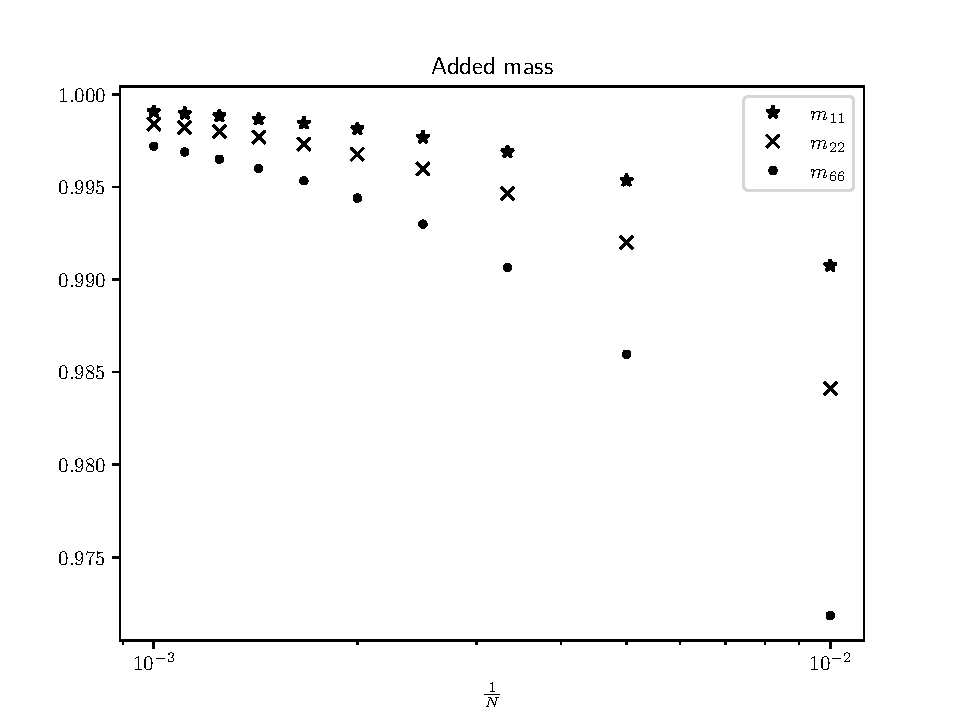
\includegraphics[width = \textwidth]{addedmass_a2_b1_N1000.pdf}
    \captionof{figure}{Addert masse for ellipse med $\sfrac{a}{b} = 2$.}
    \label{fig:addedmass_a2_b1_N1000}
\end{Figure}
\begin{Figure}
    \centering
    \captionsetup{type = figure}
    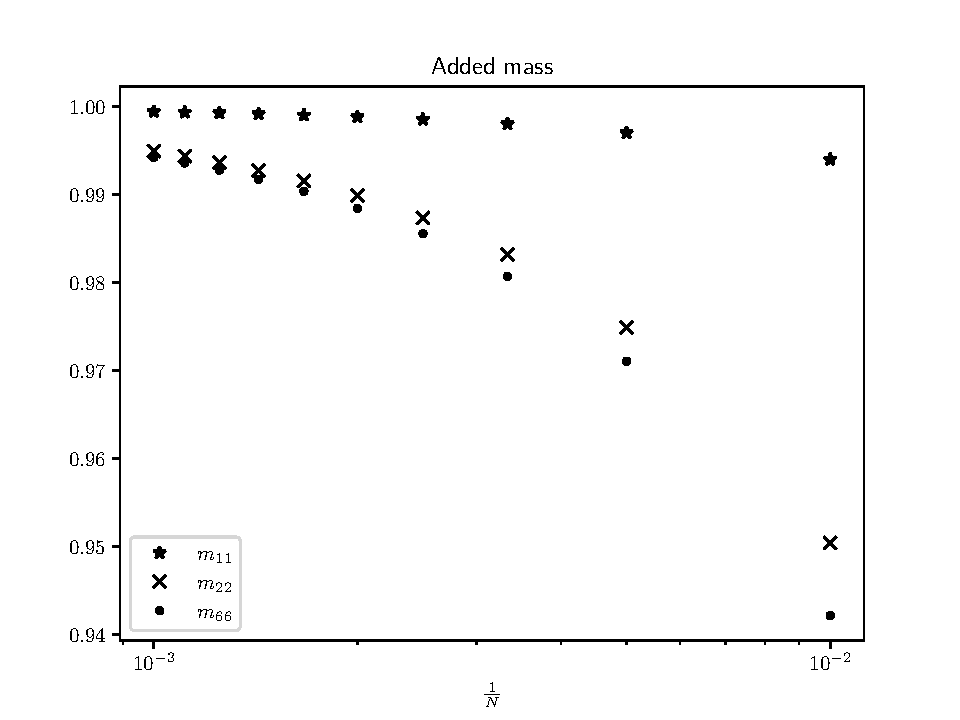
\includegraphics[width = \textwidth]{addedmass_a10_b1_N1000.pdf}
    \captionof{figure}{Addert masse for ellipse med $\sfrac{a}{b} = 10$.}
    \label{fig:addedmass_a10_b1_N1000}
\end{Figure}

\noindent Den dårligere konvergensen for større $a$ kan være grunnet større mellomrom mellom nodene.
Siden disse nodene faller nedenfor den faktiske ellipsebuen, vil normalvektoren heller ikke være helt riktig.
Dessuten vil diskretiseringen til en sirkel alltid være en regulær flerkant, hvis normalvektorer nødvendigvis peker inn mot origo, som forklarer hvorfor konvergensen er dårligere enn sirkelen.
Her ser vi ut til å ha den samme konvergensraten, med at en dobling i $N$ tilsvarer en fjerdedel av relativ feil.

Vi blir ikke spurt om å sammenlikne det numeriske potensialet koden produserer med den analytiske, så vi går ut ifra at de gode resultatene vi så for sirkelen overføres til ellipsen.
\begin{Figure}
    \centering
    \captionsetup{type = figure}
    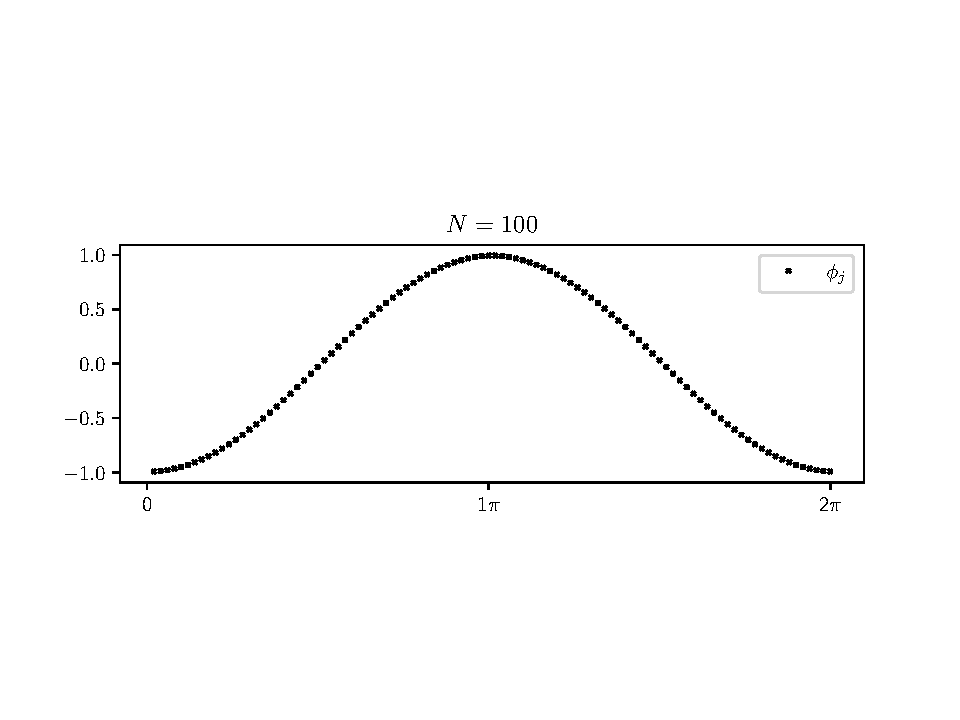
\includegraphics[width = \textwidth]{phi1_a2_b1_N100.pdf}
    \captionof{figure}{$\phi_1$ for ellipse med $\sfrac{a}{b} = 2$.}
    \label{fig:phi1_a2_b1_N100}
\end{Figure}
\begin{Figure}
    \centering
    \captionsetup{type = figure}
    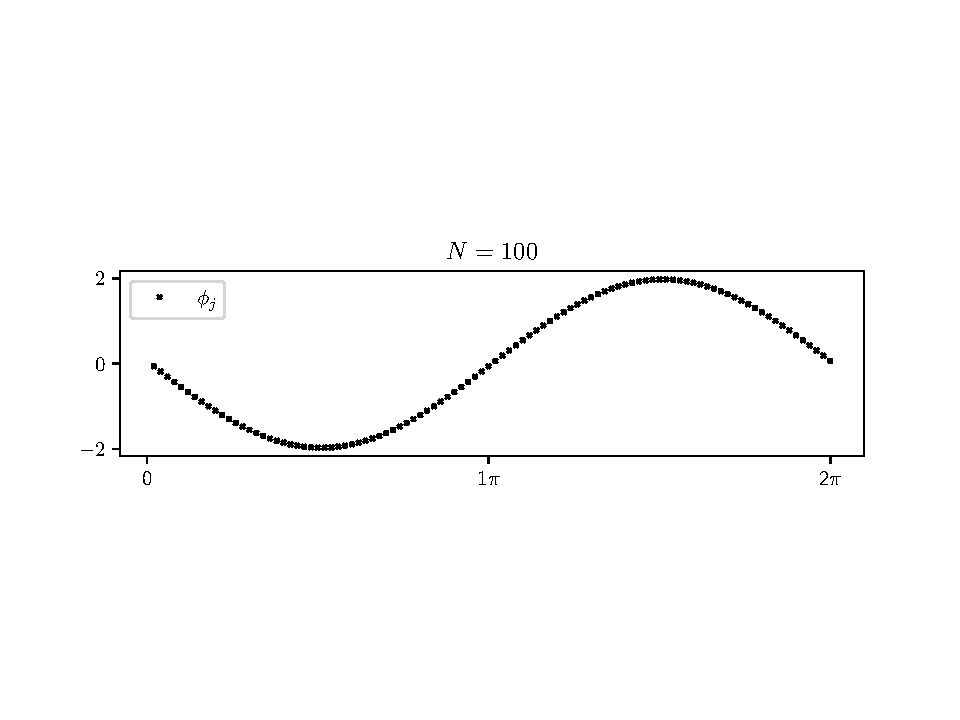
\includegraphics[width = \textwidth]{phi2_a2_b1_N100.pdf}
    \captionof{figure}{$\phi_2$ for ellipse med $\sfrac{a}{b} = 2$.}
    \label{fig:phi2_a2_b1_N100}
\end{Figure}
\begin{Figure}
    \centering
    \captionsetup{type = figure}
    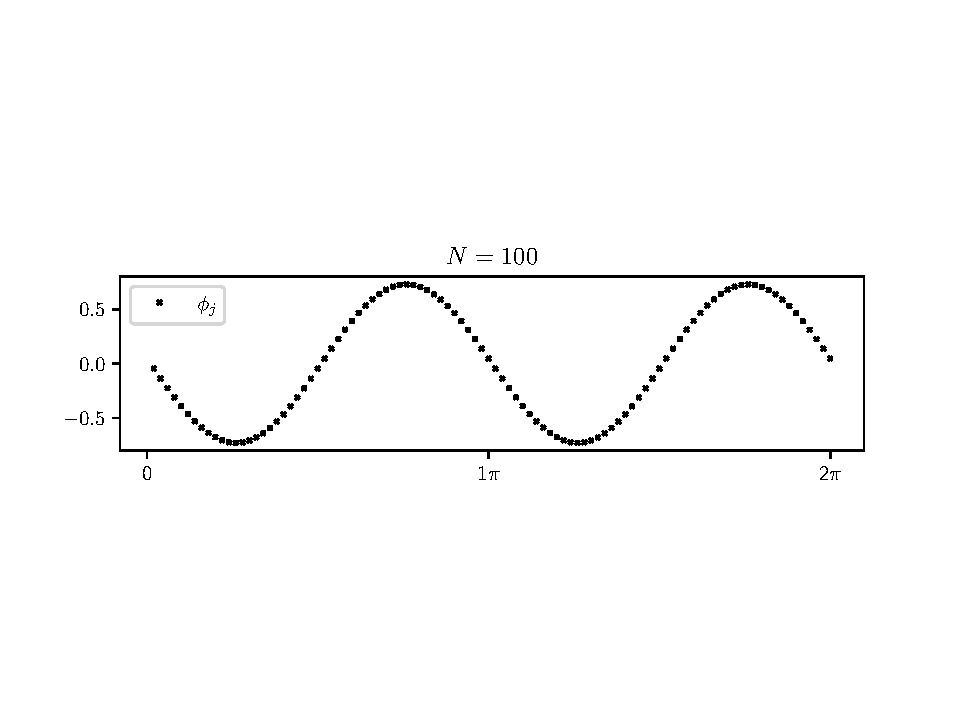
\includegraphics[width = \textwidth]{phi6_a2_b1_N100.pdf}
    \captionof{figure}{$\phi_6$ for ellipse med $\sfrac{a}{b} = 2$.}
    \label{fig:phi6_a2_b1_N100}
\end{Figure}

\begin{Figure}
    \centering
    \captionsetup{type = figure}
    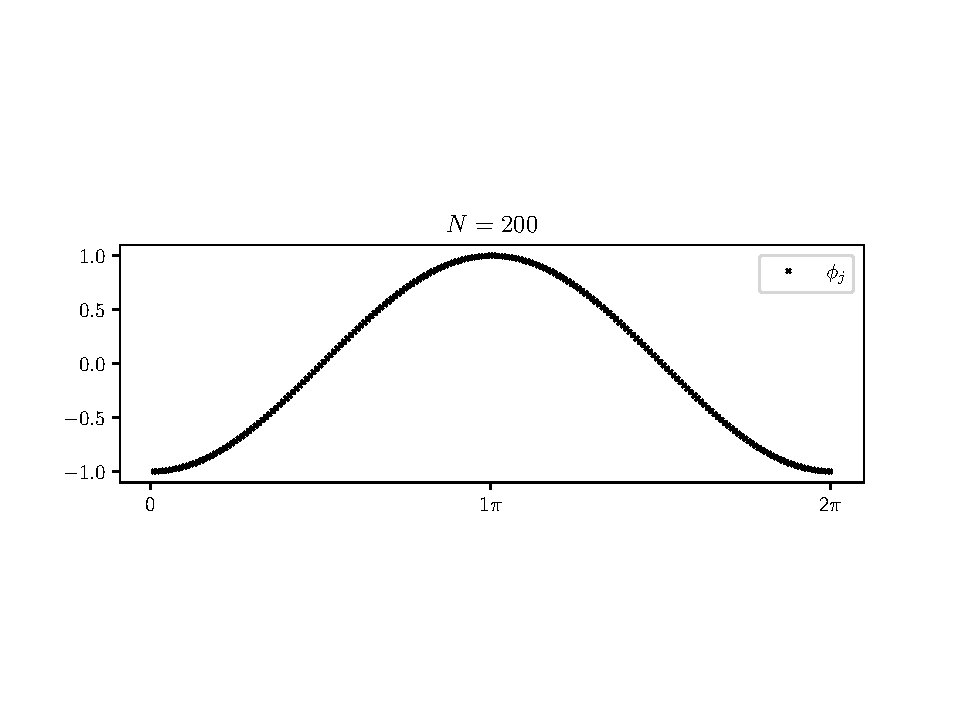
\includegraphics[width = \textwidth]{phi1_a10_b1_N200.pdf}
    \captionof{figure}{$\phi_1$ for ellipse med $\sfrac{a}{b} = 10$.}
    \label{fig:phi1_a10_b1_N200}
\end{Figure}
\begin{Figure}
    \centering
    \captionsetup{type = figure}
    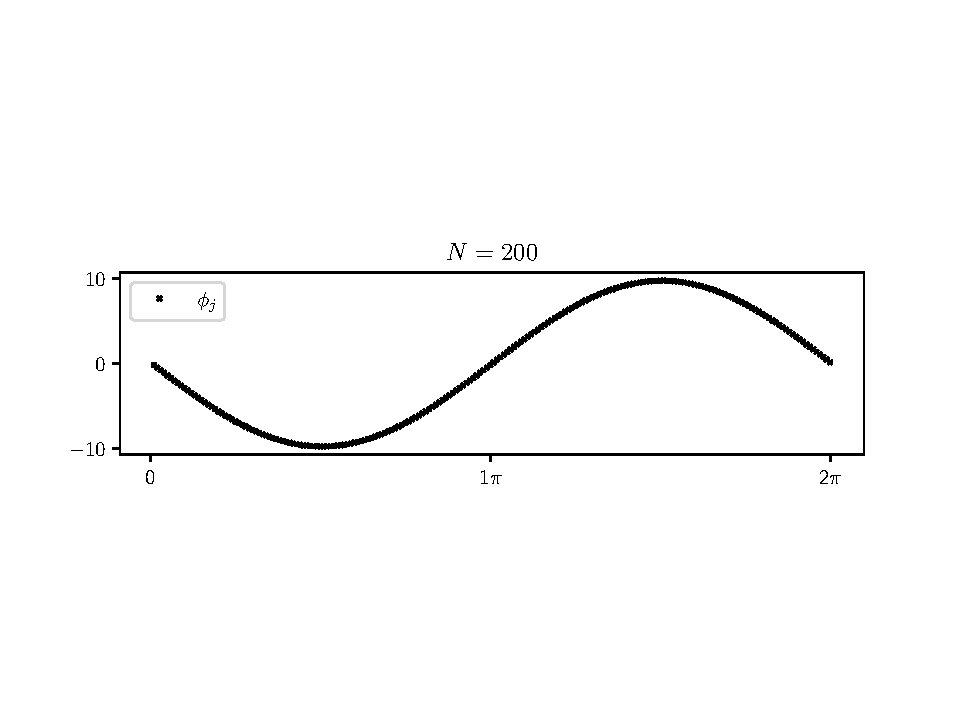
\includegraphics[width = \textwidth]{phi2_a10_b1_N200.pdf}
    \captionof{figure}{$\phi_2$ for ellipse med $\sfrac{a}{b} = 10$.}
    \label{fig:phi2_a10_b1_N200}
\end{Figure}
\begin{Figure}
    \centering
    \captionsetup{type = figure}
    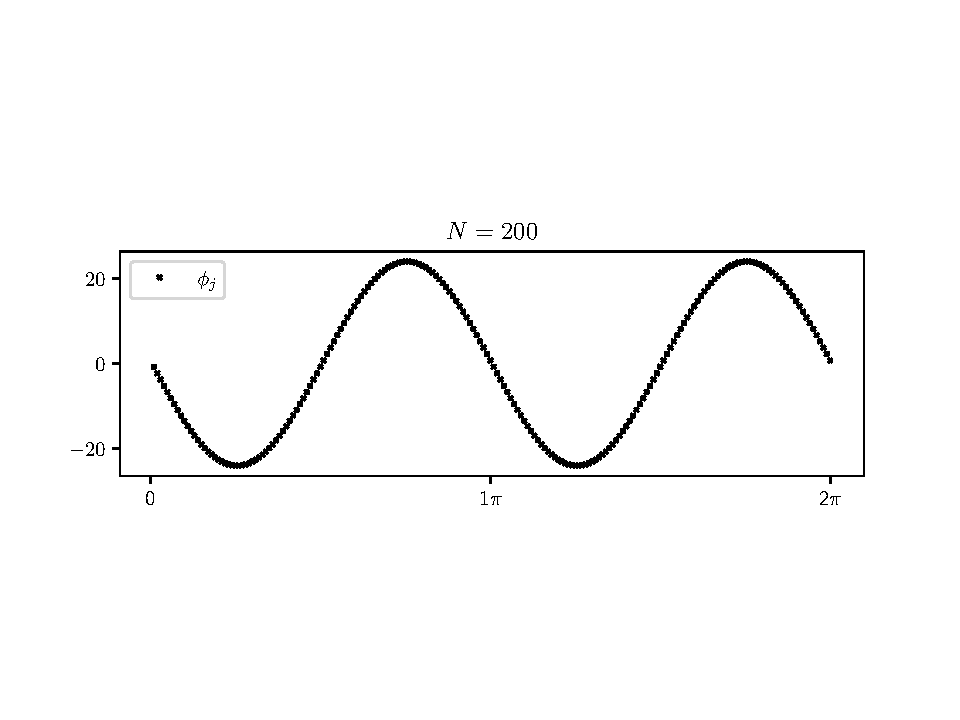
\includegraphics[width = \textwidth]{phi6_a10_b1_N200.pdf}
    \captionof{figure}{$\phi_6$ for ellipse med $\sfrac{a}{b} = 10$.}
    \label{fig:phi6_a10_b1_N200}
\end{Figure}

\noindent Amplituden til første mode ser ut til å tilsvare $b$, og andre mode $a$.